\documentclass[11pt]{article}

%Don't change any thing before \begin{document}
%They are not useful for now, but later when you try to add figures
%these might be useful. In fact if you use sth fancy, you might need
%to add more packages, or macros.
\usepackage{amssymb,amsmath}
\usepackage{times,psfrag,epsf,epsfig,graphics,graphicx}
\usepackage{algorithm}
\usepackage{algorithmic}
\usepackage{xcolor}

\begin{document}
\date{}

\title{CSCI 246: Assignment~8~(6 points)}

\author{William Jardee}

\maketitle
 
\section*{Problem 1.}

\noindent
A company offers a raffle whose grand prize is a \$60,000 new car. Additional prizes are a \$1,000 television and a \$500 computer. Tickets cost \$20 each. Ticket income will be donated to a charity. If 3,000 tickets are sold, what is the expected gain or loss (in dollars) of each ticket? (Round your answer to the nearest cent.)
\newline
\newline
\newline
\noindent
{\bf Answer:}
\[\$20 \times 3,000 = \$60,000\]
\[\$60,000 - (\$60,000 + \$1,000 + \$500) = - \$1,500\]
\[\frac{-\$1,500}{3,000} = -\frac{\$1}{2} = -\$0.50\]\\
So the expected gain per a ticket owner is $\$0.50$, the company should expect to lose $\$0.50$ per a ticket.
\newpage

\section*{Problem 2.}

\noindent
One urn contains {\color{red}9} blue balls and {\color{red}12} white balls, and a second urn contains {\color{red}12} blue balls and {\color{red}8} white balls. An urn is selected at random, and a ball is then randomly chosen from the
urn. (Round your answers to one decimal place.)
\newline

\noindent
(2.1) What is the probability (as a \%) that the chosen ball is blue?
\newline
\newline
\newline
\noindent
{\bf Answer:}~~\\

$P(A\cup B) = P(A) + P(B) - P(A\cap B)$:
\[P(b_1 \cup b_2) = 0.5\cdot \Big(\frac{9}{21}\Big) + 0.5 \cdot \Big(\frac{12}{20}\Big) - 0= 51\%\]
\newline

\noindent
(2.2) If the chosen ball is blue, what is the probability (as a \%) that it
came from the first urn?
\newline
\newline

\noindent
{\bf Answer:}\\

We want to use $P(B|A) = \frac{P(A\cap B)}{P(A)}$ which turns into $P(1|b) = \frac{P(1 \cap b)}{P(b)}$
\[P(1|b) = \frac{0.5 \cdot \frac{9}{21}}{0.514} = 41.7\%\]
\newpage


\section*{Problem 3.}

\noindent
Prove that at a party with at least two people, there are at least two mutual
acquaintances or at least two mutual strangers.
\newline
\newline
\newline
\newline
\newline
\noindent
{\bf Answer:}\\

Let the list of part members exist in a graph G were each vertex is a party-goer and each edge is an acquaintance between the two vertices. We will define the term "mutually acquaintances" as two vertices on this graph that are connect through a walk. Being "mutual strangers" is defined as not having an edge between the two points. Having at least one edge between two points is a binary condition, either there is or their is not one, meaning that these are the only two possibilities that are mutually disjoint. Let there be two vertices in the graph. As just claimed, either the two are connected by an edge or they are not. Meaning if there are two mutual acquaintances or two mutual strangers. If we add more vertices, the condition of an edge between these two original points doesn't change. This means, independent of size, there is at least one edge or no edges between the initial two vertices and there are always at least two mutual acquaintances or at least two mutual strangers.
\begin{flushright}$\blacksquare$\end{flushright}

\newpage

\section*{Problem 4.}

List the adjacency matrices for the following two graphs.
\newline

\begin{figure}[htbp]
\begin{center}
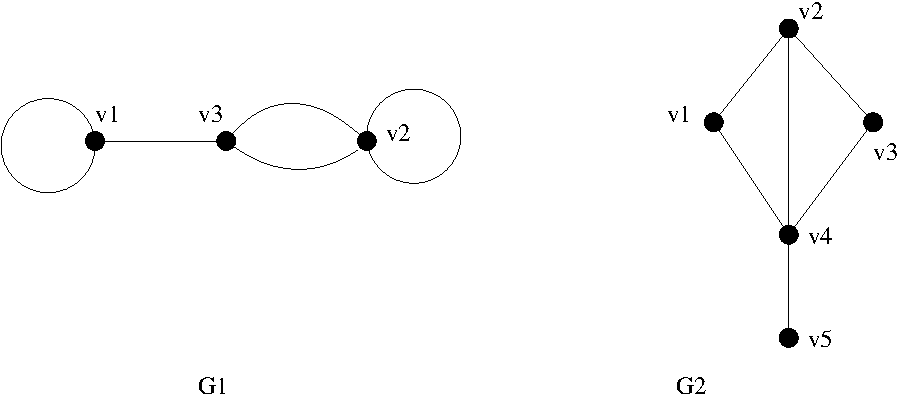
\includegraphics[scale=0.70]{fig1.pdf}
\end{center}
\label{fig1}
\caption{\bf Two graphs $G_1$ and $G_2$.}
\end{figure}
%
\noindent
{\bf Answer:}\\\\

G1:
$\begin{bmatrix}
1 & 0 & 1\\
0 & 1 & 2\\
1 & 2 & 0
\end{bmatrix}$\\\\

G2: 
$\begin{bmatrix}
0 & 1 & 0 & 1 & 0\\
1 & 0 & 1 & 1 & 0\\
0 & 1 & 0 & 1 & 0\\
1 & 1 & 1 & 0 & 1\\
0 & 0 & 0 & 1 & 0
\end{bmatrix}
$
\newline
\newpage

\section*{Problem 5.}

Consider the following description of a graph:
\newline

  Graph, circuit-free, seven vertices, four edges.
\newline

\noindent
Can such a graph exist? If so, draw an example. If not, explain the reason.
\newline
\newline
\newline
\newline

\begin{figure}[htbp]
\begin{center}
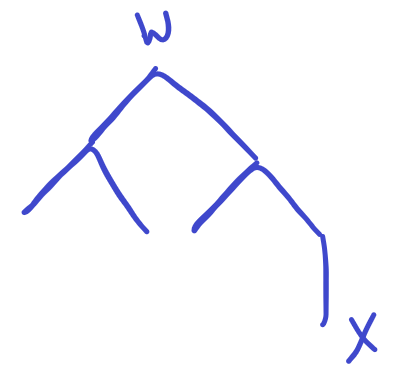
\includegraphics[scale=0.7]{Homework/graph1.png}
\end{center}
\label{fig2}
\caption{\bf Seven vertices, four edges}
\end{figure}

\end{document}
